\section{函数值反馈}
\label{sec:zo-feedback}

调节仿真器参数时，算法与仿真器之间到底交换什么信息？同样叫“只能读函数值”，读数是否带噪声、一轮能读几个位置、两次读数能否共用一次仿真，会让后面的误差结论相差几个量级。所以先把接口固定下来。

\paragraph{目标、查询点与读数}
我们要最小化$f(\bm{x})$，$\bm{x}\in\bm{C}\subseteq\mathbb{R}^n$。算法每次提交一个\term{查询点}（query point）$\bm{q}\in\mathbb{R}^n$，黑箱返回一个实数$y$，称为\term{读数}（reading）。查询点不一定等于当前迭代点，算法常常故意偏离当前点一点，再比较读数。

这里出现两种性质不同的随机性，如图~\ref{fig:zo-feedback}所示。第一种在算法内部：算法自己抽取偏离的方向，这是我们主动加入的。第二种在黑箱内部：同一个查询点运行两次，可能因为测量噪声或仿真种子不同而得到不同的读数，这是我们无法控制的。

\begin{BookInlineFigure}
  \centering
  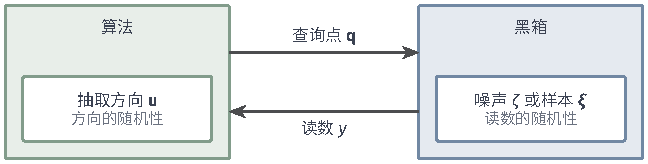
\includegraphics[width=110mm]{figures/05-optimization/05-stochastic-optimization/tikz/zo-feedback/figure.pdf}
  \caption{零阶优化的接口。算法提交查询点$\bm{q}$，黑箱返回读数$y$。方向$\bm{u}$的随机性由算法产生，噪声$\zeta$或样本$\bm{\xi}$的随机性来自黑箱，二者相互独立地起作用，分析时分别记录。}
  \label{fig:zo-feedback}
\end{BookInlineFigure}

\subsection{精确函数值与含噪读数}
\label{sec:zo-readings}

按黑箱内部的情况，读数分成三种模型。图~\ref{fig:zo-readings}画出了它们在一条一元曲线上的样子。

\paragraph{三种读数模型}
第一种是精确函数值，同一点读多少次都是同一个数：
\begin{equation}
 y=f(\bm{q}).
 \label{eq:zo-reading-exact}
\end{equation}
第二种是带\term{加性噪声}（additive noise）的读数，真实值上叠加一个随机误差$\zeta$：
\begin{equation}
 y=f(\bm{q})+\zeta.
 \label{eq:zo-reading-additive}
\end{equation}
第三种是期望目标的样本函数值。目标本身定义成随机函数的平均，一次读数对应一个随机场景$\bm{\xi}$：
\begin{equation}
 f(\bm{x})=\mathbb{E}_{\bm{\xi}}\bigl[F(\bm{x};\bm{\xi})\bigr],\qquad
 y=F(\bm{q};\bm{\xi}).
 \label{eq:zo-reading-sample}
\end{equation}

后两种的差别在于噪声是否依赖位置。贯穿例上取样本函数$F(\bm{x};\bm{\xi})=f(\bm{x})+\bm{\xi}^\top\bm{x}$，$\bm{\xi}$均值为零。场景$\bm{\xi}=(0.2,-0.1)$在起点给出
\[
 F(\bm{x}^{(0)};\bm{\xi})=45+0.2\cdot9-0.1\cdot1=46.7.
\]
这里偏差$1.7$随$\bm{x}$线性变化。固定一个场景，$F(\cdot;\bm{\xi})$是一条完整的曲线，如图~\ref{fig:zo-readings}(c)；而加性噪声模型里每次读数的误差是孤立的一个数，没有“这条曲线”可言。

\begin{BookInlineFigure}
  \centering
  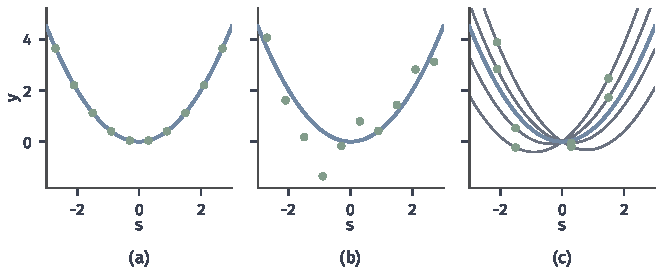
\includegraphics[width=112mm]{figures/05-optimization/05-stochastic-optimization/matplotlib/zo-readings/figure.pdf}
  \caption{同一个目标$s^2/2$（蓝线）的三种读数，绿点是读数。(a)精确读数落在曲线上。(b)加性噪声读数在曲线上下散开，标准差$0.6$。(c)样本函数$s^2/2+\xi s$，取四个场景$\xi$（灰线），绿点是同一场景曲线上的读数，蓝线是它们的期望。}
  \label{fig:zo-readings}
\end{BookInlineFigure}

\paragraph{无偏须对给定的历史和查询点成立}
什么叫“读数没有系统偏差”？直观要求是平均起来等于真值。但这个平均必须在“算法已经知道的一切”都固定时计算，否则算法可能恰好挑中噪声偏低的位置。记$\mathcal{H}$为提交本次查询之前算法产生的全部方向和读数。

\begin{definition}[条件无偏读数]
\label{def:zo-unbiased-reading}
读数$y$在查询点$\bm{q}$处称为\term{条件无偏}（conditionally unbiased）的，如果
\begin{equation}
 \mathbb{E}\bigl[y\mid\mathcal{H},\bm{q}\bigr]=f(\bm{q}).
 \label{eq:zo-conditional-unbiased}
\end{equation}
其方差有界是指：给定$\mathcal{H}$和$\bm{q}$时，$y$的条件方差不超过某个常数$\sigma^2<\infty$。
\end{definition}

条件期望可以理解为：把算法手里的信息看作已知常数，只对尚未发生的随机性求平均。严格定义可参考\BookChapterRef{chap:conditional-expectation}{卷七第4章“条件期望与条件分布”}，本章只用这一层含义和逐层取期望的规则。

边际无偏是不够的。设两个候选的真实值都是$0$，噪声等可能取$\pm1$，每个候选的噪声一旦生成就不再变化。先各读一次，然后挑读数较低的候选再读一次。第一次读数的边际均值是$0$，第二次读数却满足：
\[
 \mathbb{P}(\text{第二次读数}=-1)=\frac34,\qquad
 \mathbb{P}(\text{第二次读数}=+1)=\frac14.
\]
第二次读数的均值是$-\tfrac12$，而被选中候选的真值是$0$。噪声与“查询哪里”发生了关联，式~\eqref{eq:zo-conditional-unbiased}不成立。这说明重复使用同一份噪声时，查询点不能依赖这份噪声生成的读数。

\paragraph{目标确定时也可以用随机方向}
“随机优化”容易让人以为目标必须是随机的，其实不然。贯穿例~\eqref{eq:zo-example}若采用模型~\eqref{eq:zo-reading-exact}，黑箱完全确定。算法仍可以抽方向$\bm{u}=(0.6,0.8)$，查询$\bm{x}^{(0)}\pm0.5\bm{u}$，得到
\[
 f(9.3,1.4)=52.065,\qquad f(8.7,0.6)=39.465.
\]
重读多少次这两个数都不变，唯一的随机性是方向。反过来，若固定方向沿坐标轴逐个差分而读数带噪声，随机性就全部来自黑箱。两种随机性可以单独出现，也可以同时出现，分析时分开记录。

\subsection{单点查询与成对查询}
\label{sec:zo-pair-interface}

读数的模型说的是一次读数的性质，还需要规定多次读数之间的关系。这里有两个相互独立的问题。

\paragraph{一轮能读几个位置}
有些系统每次只能在一组参数下运行，下一轮参数已经变了，同一状态无法读第二个位置。这称为\term{单点查询}（single-point query）。另一些系统允许在同一轮提交两个位置，比如对称地偏离当前点，这称为\term{成对查询}（paired query）。前者更受限，后者能够比较两个读数，这是一项实质性的额外能力，不是实现细节。

\paragraph{两个位置能否共用一次仿真}
成对查询时还要问：两次读数用的是不是同一个随机场景？比如仿真器允许固定随机种子，那么可以读
\begin{equation}
 y_+=F(\bm{q}_+;\bm{\xi}),\qquad y_-=F(\bm{q}_-;\bm{\xi}),
 \label{eq:zo-shared-pair}
\end{equation}
也就是沿同一条样本曲线读两点。这称为\term{共享样本}（shared sample），又叫共同随机数。如果种子无法控制，两个读数各带独立的噪声：
\begin{equation}
 y_+=f(\bm{q}_+)+\zeta_+,\qquad y_-=f(\bm{q}_-)+\zeta_-.
 \label{eq:zo-independent-pair}
\end{equation}

\paragraph{为什么不能混为一谈}
两个模型的读数单独看可能分布完全相同，算差却完全不同。图~\ref{fig:zo-pair-readings}取$f(s)=s^2/2$，在$s=1$两侧相距$0.4$读两点，真实导数是$1$。左边噪声独立，分别取$+0.3$和$-0.3$，差商是
\[
 \frac{y_+-y_-}{2\cdot0.4}=\frac{(0.98+0.3)-(0.18-0.3)}{0.8}=1.75.
\]
右边两点共享噪声$+0.3$，差商里这个数被减掉，得到准确的$1$。相同大小的噪声，一边造成$75\%$的误差，一边没有影响。

\begin{BookInlineFigure}
  \centering
  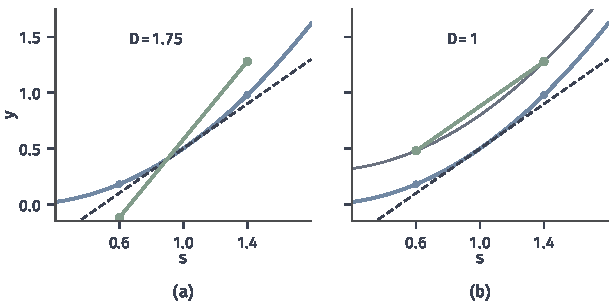
\includegraphics[width=104mm]{figures/05-optimization/05-stochastic-optimization/matplotlib/zo-pair-readings/figure.pdf}
  \caption{成对读数的两种接口，蓝线为$f(s)=s^2/2$，虚线是$s=1$处的切线，绿色线段连接两次读数，蓝点是真实函数值。(a)两点噪声独立，分别为$+0.3$和$-0.3$，线段斜率$1.75$，偏离切线。(b)两点共享噪声$+0.3$，读数都落在灰色曲线上，斜率恰为$1$。}
  \label{fig:zo-pair-readings}
\end{BookInlineFigure}

所以误差界必须与实际接口匹配。文献和本章后面给出的速率都带着接口条件，表~\ref{tab:zo-interfaces}先列出本章要用到的四种情形，第~\ref{sec:zo-pair-noise}节再推导对应的方差。

\begin{BookInlineTable}
  \centering
  \begin{tabular}{@{}lll@{}}
    \toprule
    接口 & 一轮读数 & 两点之差的噪声\\
    \midrule
    精确函数值 & 任意 & 无\\
    单点，含噪 & $1$ & 不适用\\
    成对，独立噪声 & $2$ & 方差$2\sigma^2$，不随距离变小\\
    成对，共享样本 & $2$ & 取决于样本函数的波动\\
    \bottomrule
  \end{tabular}
  \caption{本章区分的查询接口。“独立噪声”指式~\eqref{eq:zo-independent-pair}，噪声方差为$\sigma^2$；“共享样本”指式~\eqref{eq:zo-shared-pair}。}
  \label{tab:zo-interfaces}
\end{BookInlineTable}
